% Single side-view option A: vertical left edge; all 5 segments solid.
% Vertices E (bottom-left), T (top-left), B (top), R (bottom-right); diagonal E-B.
% Original "(A)" is the choice enumerator outside the geometry and is not redrawn.
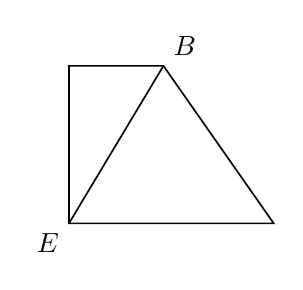
\begin{tikzpicture}[line width=.6pt,font=\normalsize,x=1cm,y=1cm]
\coordinate (E) at (0,0);
\coordinate (T) at (0,2);
\coordinate (B) at (1.2,2);
\coordinate (R) at (2.6,0);
\draw (E) -- (T) -- (B) -- (R) -- cycle;
\draw (E) -- (B);
\node[below left] at (E) {$E$};
\node[above right] at (B) {$B$};
\end{tikzpicture}
